%!TEX root = ../thesis.tex

%%%%%%%%%%%%%%%%%%%%%%%%%%%%%%%%%%%%%%%%%%%%%%%%%%%%%%
%%%%%%%%%%%%%%%%%%%%%%%%%%%%%%%%%%%%%%%%%%%%%%%%%%%%%%
\subsection{SAJaS}
\begin{frame}{SAJaS}
	Acções dos agentes são ecapsuladas em ``Behaviours''
	\begin{figure}[h]
		\centering
		\includegraphics[height=7cm]{../figures/jade_fluxogram.pdf}
		\label{fig:jade_fluxogram}
	\end{figure}
\end{frame}
\begin{frame}{SAJaS}
	
\end{frame}
\begin{frame}{SAJaS}
	Duas alternativas para execução
	\begin{figure}[H]
		\centering
	    \begin{subfigure}[b]{.45\linewidth}
			\centering
			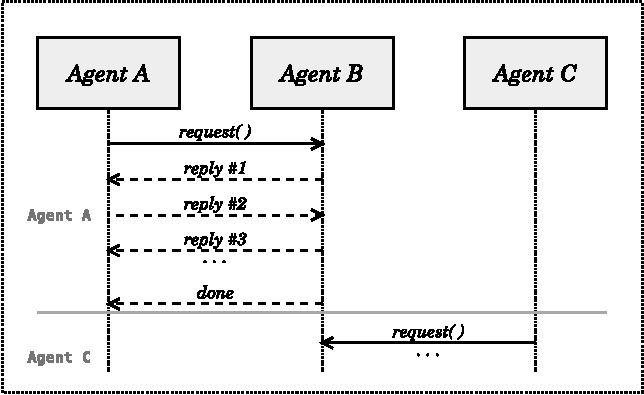
\includegraphics[width=\linewidth]{../figures/executionProblem.pdf}
			\caption{\small Acesso Direto}
			\label{fig:direct_method_execution}
	    \end{subfigure}
	    \begin{subfigure}[b]{.45\linewidth}
			\centering
			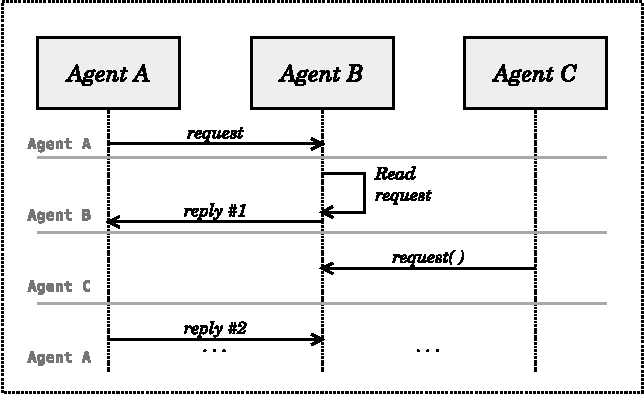
\includegraphics[width=\linewidth]{../figures/executionProblem2.pdf}
			\caption{\small Assíncrono}
			\label{fig:assynch_execution}
	    \end{subfigure}
	    \label{fig:execution_problems}
	\end{figure}

\end{frame}
\begin{frame}{SAJaS}
	Solução para communicação ``assíncrona'' no SAJaS
	\begin{figure}
		\centering
	    \begin{subfigure}[b]{0.45\linewidth}
			\centering
			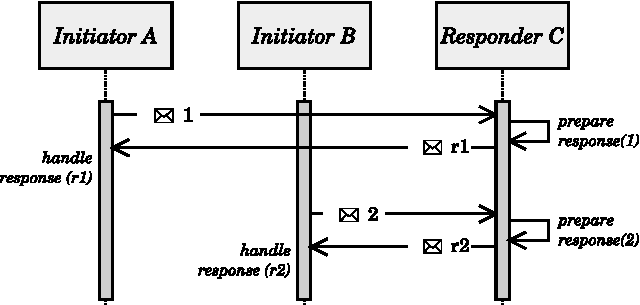
\includegraphics[width=\linewidth]{../figures/tickExample2.pdf}
			\caption{JADE}
			\label{fig:com-example-jade}
	    \end{subfigure}
	    \begin{subfigure}[b]{0.45\linewidth}
			\centering
			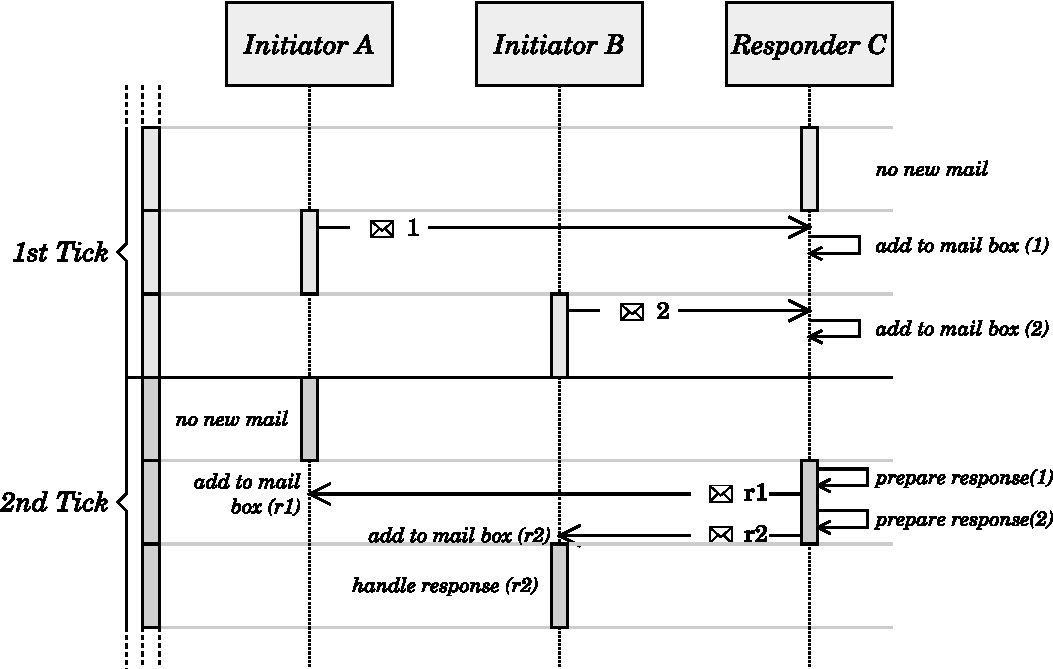
\includegraphics[width=\linewidth]{../figures/tickExample.pdf}
			\caption{SAJaS}
			\label{fig:com-example-repast}
	    \end{subfigure}
	    \caption{Communication and agent interaction}
	    \label{fig:execution_example}
	\end{figure}

\end{frame}

\subsection{Arquitetura}
\begin{frame}{Arquitetura}

\end{frame}

\subsection{FIPA}
\begin{frame}{FIPA}

\end{frame}